\documentclass[border={5pt 5pt 5pt 5pt}, preview]{standalone}

% Math & Symbol packages
\usepackage{amsmath}
\usepackage{amssymb}

% Graphics & Float packages
\usepackage{float}
\usepackage{graphicx}
\usepackage{subfigure}
\usepackage{tikz}
\usepackage{pgfplots}
\usetikzlibrary{patterns, arrows.meta, calc}
\pgfplotsset{compat=newest}
\usepgfplotslibrary{fillbetween}

% Colors
\usepackage{xcolor}
\definecolor{HMSRed}{HTML}{C5112E}  % [197, 17, 46]
\definecolor{MGHBlue}{HTML}{008BB0} % [0, 139, 176]
\definecolor{MGHGrey}{HTML}{626365} % [98, 99, 101]

\begin{document}

% KvA: Example Figure, didn't care too much about efficiency
\begin{figure}[htp]
\centering
    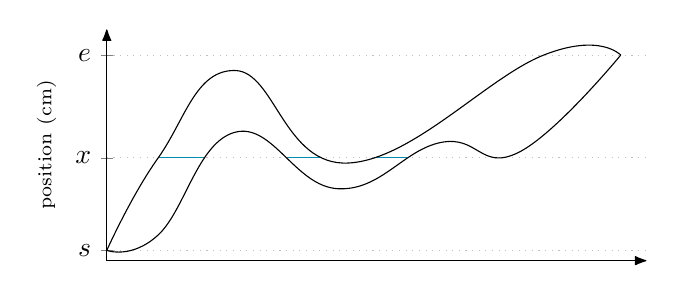
\begin{tikzpicture}[remember picture]
        \pgfplotsset{holdot/.style={color=black,only marks,mark=*,mark size=1.5pt}}
        \pgfplotsset{soldot/.style={color=white,only marks,mark=*,mark size=1.5pt}}
        \begin{axis}[
            xmin=0, xmax=10.50,
            ymin=0, ymax=4.5,
            grid = both,
            grid style = dotted,
            axis x line = bottom,
            axis y line = left,
            enlargelimits = {abs=0.0},
            axis line style = {-Latex[round]},
            yticklabels = {$s$,$x$,$e$},
            ytick = {0.2,2,4},
            xtick = \empty,
            ylabel = {\scriptsize{position (cm)}},
            axis equal image
        ]

            % Vertical lines (top)
            \node[] (traj-1) at (axis cs:1,4.2) {};
            \node[] (traj-2) at (axis cs:1.88,4.2) {};
            \node[] (traj-3) at (axis cs:3.5,4.2) {};
            \node[] (traj-4) at (axis cs:4.17,4.2) {};
            \node[] (traj-5) at (axis cs:5.2,4.2) {};
            \node[] (traj-6) at (axis cs:5.85,4.2) {};
            \node[] (traj-10) at (axis cs:10,4.2) {};

            % Exposure times
            \draw[MGHBlue] (1,2) -- (1.89,2);
            \draw[MGHBlue] (3.5,2) -- (4.17,2.0);
            \draw[MGHBlue] (5.2,2) -- (5.85,2);

            % Leaf trajectories
            \addplot[name path global = leafl, black, smooth, tension=0.75] coordinates{(0,0.2)(1,2)(2.5,3.7)(4.7,1.9)(8.5,4)(10,4)};
            \addplot[name path global = leafr, black, smooth, tension=0.75] coordinates{(0,0.2)(1,0.5)(2.5,2.5)(4.5,1.4)(6.5,2.3)(8,2.1)(10,4)};

        \end{axis}
    \end{tikzpicture}

    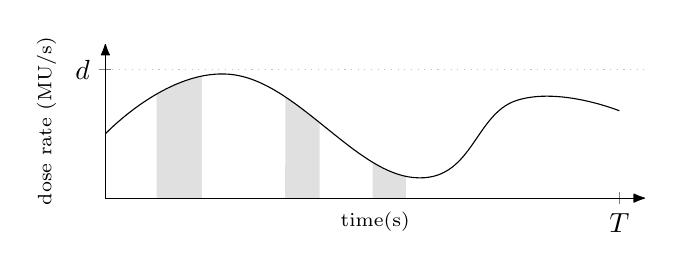
\begin{tikzpicture}[remember picture]
        \pgfplotsset{holdot/.style={color=black,only marks,mark=*,mark size=1.5pt}}
        \pgfplotsset{soldot/.style={color=white,only marks,mark=*,mark size=1.5pt}}
        \begin{axis}[
            xmin=0, xmax=10.50,
            ymin=0, ymax=3.0,
            ymajorgrids = true,
            grid style = dotted,
            axis x line = bottom,
            axis y line = left,
            enlargelimits = {abs=0.0},
            axis line style = {-Latex[round]},
            xticklabels = {$T$},
            xtick = {10},
            yticklabels = {$d$},
            ytick = {2.5},
            xlabel style = {at={(ticklabel* cs:0.5,1.5)},anchor=north},
            xlabel = {\scriptsize{time(s)}},
            ylabel = {\scriptsize{dose rate (MU/s)}},
            axis equal image
        ]

            % Vertical lines (bottom)
            \node[] (dose-1) at (axis cs:1,-0.2) {};
            \node[] (dose-2) at (axis cs:1.88,-0.2) {};
            \node[] (dose-3) at (axis cs:3.5,-0.2) {};
            \node[] (dose-4) at (axis cs:4.17,-0.2) {};
            \node[] (dose-5) at (axis cs:5.2,-0.2) {};
            \node[] (dose-6) at (axis cs:5.85,-0.2) {};
            \node[] (dose-10) at (axis cs:10,-0.2) {};

            % Dose rate pattern
            \addplot[name path global = dose, black, smooth, tension=0.75] coordinates{(0,1.25)(2.5,2.4)(6,0.4)(8,1.9)(10,1.7)};\
            \addplot[name path global = xaxis, draw=none, domain=0:11] {0};

            % Integrals
            \addplot [thick, color=blue, fill=MGHGrey, fill opacity=0.2]
                fill between[of=xaxis and dose, soft clip={domain=1:1.88}];
            \addplot [thick, color=blue, fill=MGHGrey, fill opacity=0.2]
                fill between[of=xaxis and dose, soft clip={domain=3.5:4.17}];
            \addplot [thick, color=blue, fill=MGHGrey, fill opacity=0.2]
                fill between[of=dose and xaxis, soft clip={domain=5.2:5.85}];

            % Correction
            \addplot[fill = white]
                fill between[of=xaxis and dose, soft clip={domain=1.88:2}]; % filling
            \addplot[fill = white]
                fill between[of=xaxis and dose, soft clip={domain=4.17:4.5}]; % filling
            \addplot[fill = white]
                fill between[of=xaxis and dose, soft clip={domain=5.85:6}]; % filling
             \draw[black] (0,0) -- (10,0);

        \end{axis}
    \end{tikzpicture}

    \begin{tikzpicture}[remember picture,overlay]
        \draw[dashed,MGHGrey!60] (traj-1) -- (dose-1);
        \draw[dashed,MGHGrey!60] (traj-2) -- (dose-2);
        \draw[dashed,MGHGrey!60] (traj-3) -- (dose-3);
        \draw[dashed,MGHGrey!60] (traj-4) -- (dose-4);
        \draw[dashed,MGHGrey!60] (traj-5) -- (dose-5);
        \draw[dashed,MGHGrey!60] (traj-6) -- (dose-6);
        \draw[dashed,MGHGrey!60] (traj-10) -- (dose-10);
    \end{tikzpicture}
    
\vspace{-0.7cm}
\caption[Illustration of administered dose]{
    Illustration of administered dose: the dose administered to a position $x$ equals the integral (shaded area) of the dose rate (lower panel) over the moments in time (blue lines) that position is exposed by the leaves (upper panel).
    }
\label{fig: expint}
\end{figure}

\end{document} 